\documentclass{standalone}
\usepackage{tikz}
\usetikzlibrary{patterns, positioning}
\usepackage[sfdefault]{ClearSans} %% option 'sfdefault' activates Clear Sans as the default text font
\usepackage[T1]{fontenc}

\begin{document}
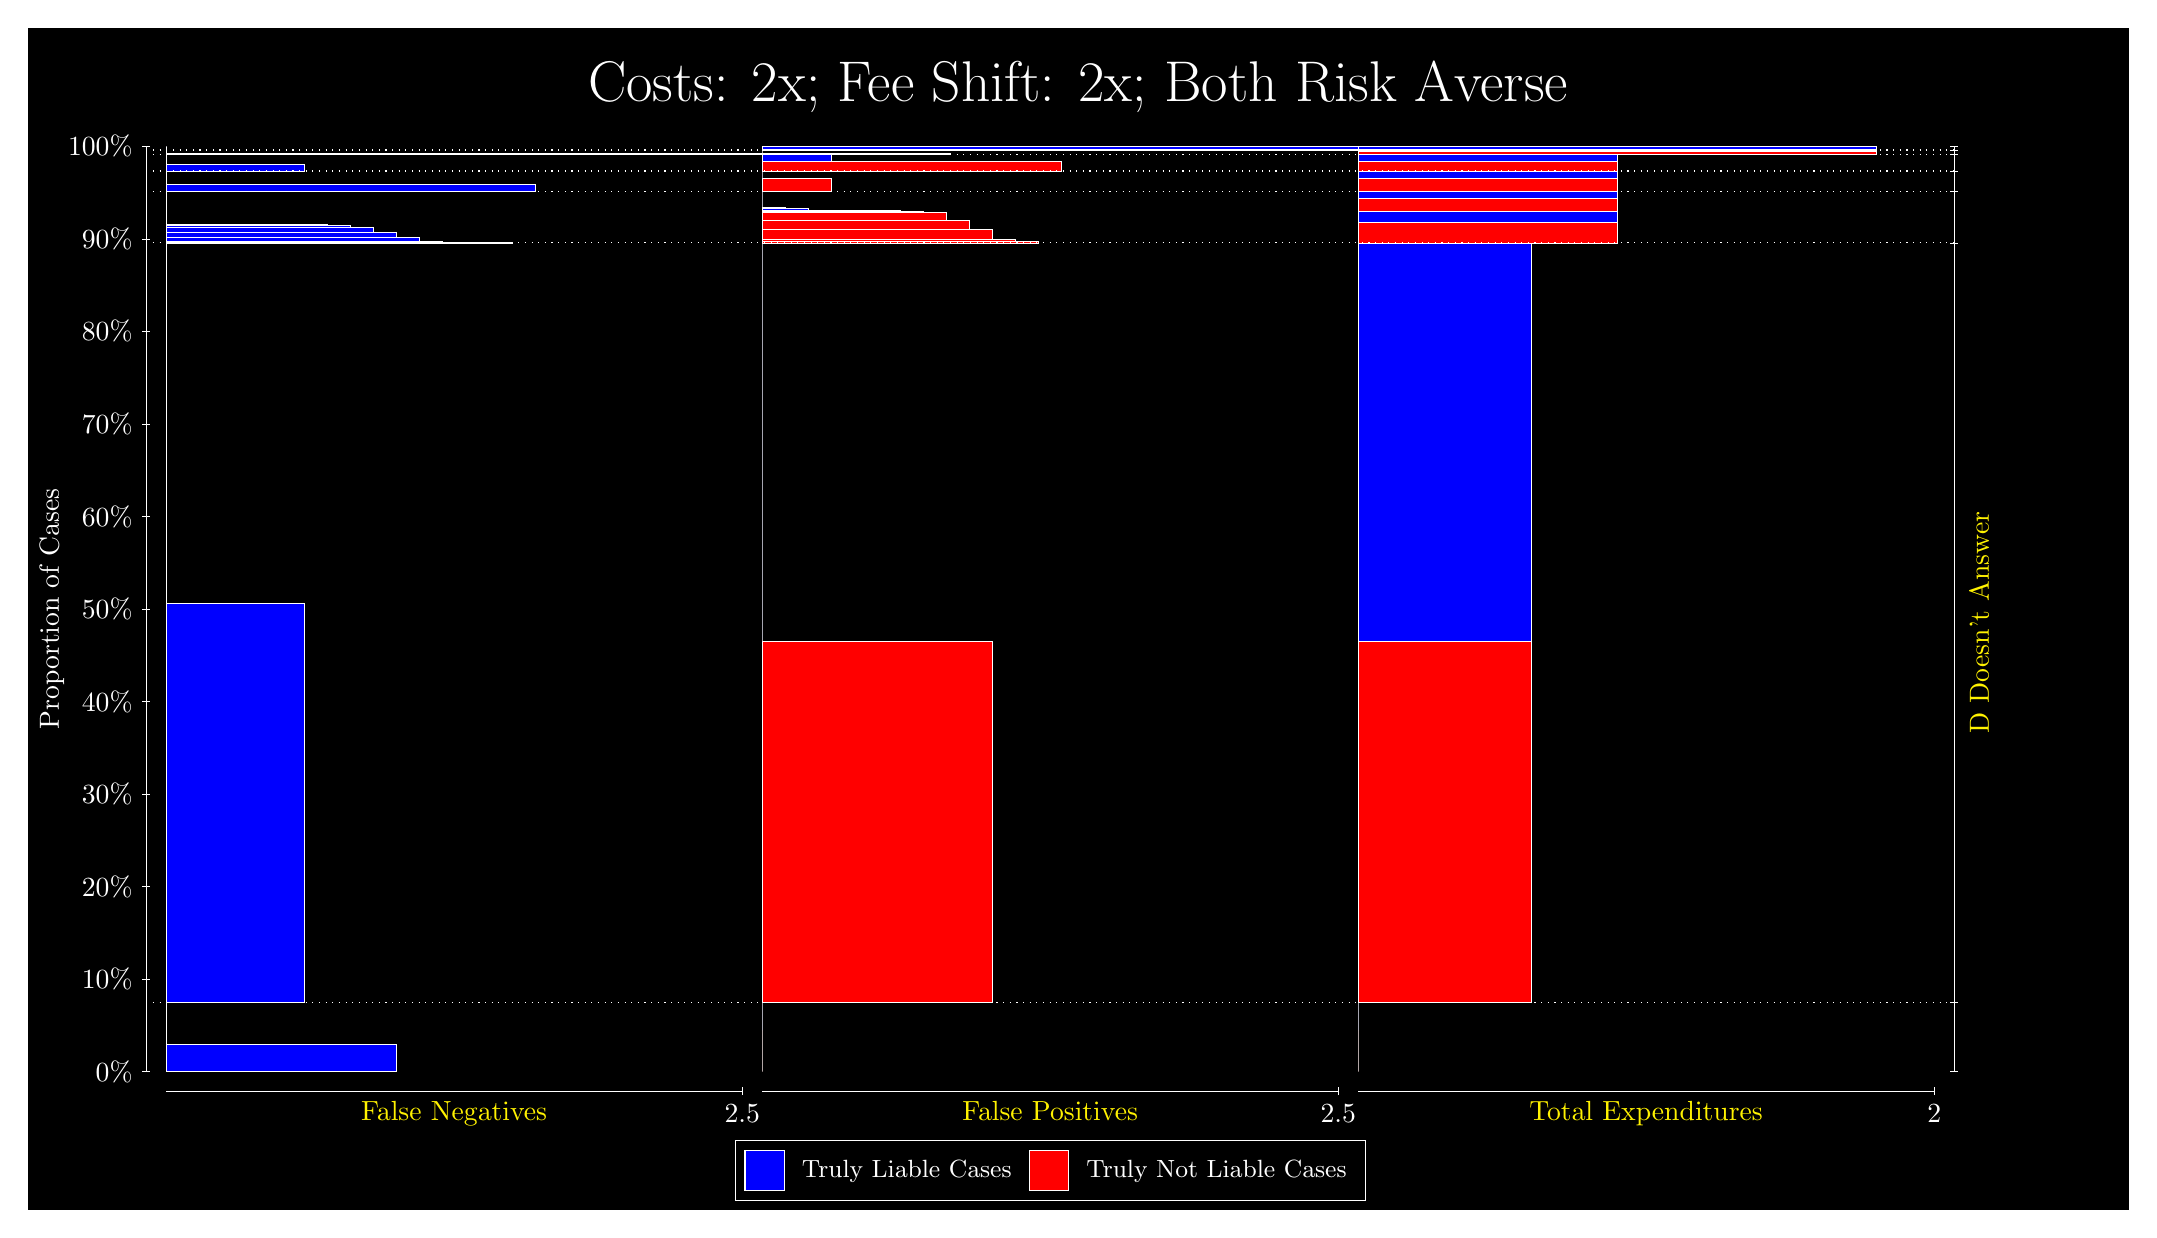
\begin{tikzpicture}
\draw[fill=black] (0,0) rectangle (26.667,15);
\draw[text=white] (0,13.5) rectangle (26.667,15) node[midway] {\huge Costs: 2x; Fee Shift: 2x; Both Risk Averse};
\draw[white, very thin] (1.5,1.75) -- (1.5,13.5);
\node[rotate=90, text=white, anchor=center] at (0.3, 7.625) {Proportion of Cases};
\draw[white, very thin] (1.45,1.75) -- (1.55,1.75);
\node[text=white, anchor=east] at (1.45, 1.75) {0\%};
\draw[white, very thin] (1.45,2.925) -- (1.55,2.925);
\node[text=white, anchor=east] at (1.45, 2.925) {10\%};
\draw[white, very thin] (1.45,4.1) -- (1.55,4.1);
\node[text=white, anchor=east] at (1.45, 4.1) {20\%};
\draw[white, very thin] (1.45,5.275) -- (1.55,5.275);
\node[text=white, anchor=east] at (1.45, 5.275) {30\%};
\draw[white, very thin] (1.45,6.45) -- (1.55,6.45);
\node[text=white, anchor=east] at (1.45, 6.45) {40\%};
\draw[white, very thin] (1.45,7.625) -- (1.55,7.625);
\node[text=white, anchor=east] at (1.45, 7.625) {50\%};
\draw[white, very thin] (1.45,8.8) -- (1.55,8.8);
\node[text=white, anchor=east] at (1.45, 8.8) {60\%};
\draw[white, very thin] (1.45,9.975) -- (1.55,9.975);
\node[text=white, anchor=east] at (1.45, 9.975) {70\%};
\draw[white, very thin] (1.45,11.15) -- (1.55,11.15);
\node[text=white, anchor=east] at (1.45, 11.15) {80\%};
\draw[white, very thin] (1.45,12.325) -- (1.55,12.325);
\node[text=white, anchor=east] at (1.45, 12.325) {90\%};
\draw[white, very thin] (1.45,13.5) -- (1.55,13.5);
\node[text=white, anchor=east] at (1.45, 13.5) {100\%};

\draw[white, very thin] (24.457,1.75) -- (24.457,13.5);
\draw[white, very thin] (24.407,1.75) -- (24.507,1.75);
\node[anchor=west] at (24.407, 1.75) {};
\draw[white, very thin] (24.407,2.6289) -- (24.507,2.6289);
\node[anchor=west] at (24.407, 2.6289) {};
\draw[white, very thin] (24.407,12.273) -- (24.507,12.273);
\node[anchor=west] at (24.407, 12.273) {};
\draw[white, very thin] (24.407,12.929) -- (24.507,12.929);
\node[anchor=west] at (24.407, 12.929) {};
\draw[white, very thin] (24.407,13.186) -- (24.507,13.186);
\node[anchor=west] at (24.407, 13.186) {};
\draw[white, very thin] (24.407,13.399) -- (24.507,13.399);
\node[anchor=west] at (24.407, 13.399) {};
\draw[white, very thin] (24.407,13.453) -- (24.507,13.453);
\node[anchor=west] at (24.407, 13.453) {};
\draw[white, very thin] (24.407,13.5) -- (24.507,13.5);
\node[anchor=west] at (24.407, 13.5) {};

\draw[white, very thin, fill=blue] (1.75,1.75) rectangle (4.6775,2.1019);
\draw[white, very thin, fill=red] (1.75,2.1019) rectangle (1.75,2.6289);
\draw[white, very thin, fill=blue] (1.75,2.6289) rectangle (3.5065,7.6935);
\draw[white, very thin, fill=red] (1.75,7.6935) rectangle (1.75,12.273);
\draw[white, very thin, fill=blue] (1.75,12.273) rectangle (6.1413,12.276);
\draw[white, very thin, fill=blue] (1.75,12.276) rectangle (5.8486,12.279);
\draw[white, very thin, fill=blue] (1.75,12.279) rectangle (5.5558,12.284);
\draw[white, very thin, fill=blue] (1.75,12.284) rectangle (5.2631,12.291);
\draw[white, very thin, fill=blue] (1.75,12.291) rectangle (4.9703,12.345);
\draw[white, very thin, fill=blue] (1.75,12.345) rectangle (4.6775,12.405);
\draw[white, very thin, fill=blue] (1.75,12.405) rectangle (4.3848,12.473);
\draw[white, very thin, fill=blue] (1.75,12.473) rectangle (4.092,12.492);
\draw[white, very thin, fill=blue] (1.75,12.492) rectangle (3.7993,12.508);
\draw[white, very thin, fill=red] (1.75,12.508) rectangle (1.75,12.929);
\draw[white, very thin, fill=blue] (1.75,12.929) rectangle (6.4341,13.018);
\draw[white, very thin, fill=red] (1.75,13.018) rectangle (1.75,13.186);
\draw[white, very thin, fill=blue] (1.75,13.186) rectangle (3.5065,13.273);
\draw[white, very thin, fill=red] (1.75,13.273) rectangle (1.75,13.399);
\draw[white, very thin, fill=blue] (1.75,13.399) rectangle (11.704,13.408);
\draw[white, very thin, fill=red] (1.75,13.408) rectangle (1.75,13.453);
\draw[white, very thin, fill=red] (1.75,13.453) rectangle (1.75,13.462);
\draw[white, very thin, fill=blue] (1.75,13.462) rectangle (1.75,13.5);
\draw[white, very thin, fill=red] (9.3189,1.75) rectangle (9.3189,2.277);
\draw[white, very thin, fill=blue] (9.3189,2.277) rectangle (9.3189,2.6289);
\draw[white, very thin, fill=red] (9.3189,2.6289) rectangle (12.246,7.2088);
\draw[white, very thin, fill=blue] (9.3189,7.2088) rectangle (9.3189,12.273);
\draw[white, very thin, fill=red] (9.3189,12.273) rectangle (12.832,12.291);
\draw[white, very thin, fill=red] (9.3189,12.291) rectangle (12.539,12.319);
\draw[white, very thin, fill=red] (9.3189,12.319) rectangle (12.246,12.441);
\draw[white, very thin, fill=red] (9.3189,12.441) rectangle (11.954,12.563);
\draw[white, very thin, fill=red] (9.3189,12.563) rectangle (11.661,12.665);
\draw[white, very thin, fill=red] (9.3189,12.665) rectangle (11.368,12.676);
\draw[white, very thin, fill=red] (9.3189,12.676) rectangle (11.075,12.685);
\draw[white, very thin, fill=red] (9.3189,12.685) rectangle (10.783,12.69);
\draw[white, very thin, fill=red] (9.3189,12.69) rectangle (10.49,12.694);
\draw[white, very thin, fill=blue] (9.3189,12.694) rectangle (9.9044,12.71);
\draw[white, very thin, fill=blue] (9.3189,12.71) rectangle (9.6116,12.73);
\draw[white, very thin, fill=blue] (9.3189,12.73) rectangle (9.3189,12.929);
\draw[white, very thin, fill=red] (9.3189,12.929) rectangle (10.197,13.097);
\draw[white, very thin, fill=blue] (9.3189,13.097) rectangle (9.3189,13.186);
\draw[white, very thin, fill=red] (9.3189,13.186) rectangle (13.125,13.312);
\draw[white, very thin, fill=blue] (9.3189,13.312) rectangle (10.197,13.399);
\draw[white, very thin, fill=red] (9.3189,13.399) rectangle (9.3189,13.443);
\draw[white, very thin, fill=blue] (9.3189,13.443) rectangle (9.3189,13.453);
\draw[white, very thin, fill=red] (9.3189,13.453) rectangle (21.029,13.462);
\draw[white, very thin, fill=blue] (9.3189,13.462) rectangle (18.102,13.5);
\draw[white, very thin, fill=red] (16.888,1.75) rectangle (16.888,2.277);
\draw[white, very thin, fill=blue] (16.888,2.277) rectangle (16.888,2.6289);
\draw[white, very thin, fill=red] (16.888,2.6289) rectangle (19.083,7.2088);
\draw[white, very thin, fill=blue] (16.888,7.2088) rectangle (19.083,12.273);
\draw[white, very thin, fill=red] (16.888,12.273) rectangle (20.181,12.53);
\draw[white, very thin, fill=blue] (16.888,12.53) rectangle (20.181,12.674);
\draw[white, very thin, fill=red] (16.888,12.674) rectangle (20.181,12.839);
\draw[white, very thin, fill=blue] (16.888,12.839) rectangle (20.181,12.929);
\draw[white, very thin, fill=red] (16.888,12.929) rectangle (20.181,13.097);
\draw[white, very thin, fill=blue] (16.888,13.097) rectangle (20.181,13.186);
\draw[white, very thin, fill=red] (16.888,13.186) rectangle (20.181,13.312);
\draw[white, very thin, fill=blue] (16.888,13.312) rectangle (20.181,13.399);
\draw[white, very thin, fill=red] (16.888,13.399) rectangle (23.475,13.443);
\draw[white, very thin, fill=blue] (16.888,13.443) rectangle (23.475,13.453);
\draw[white, very thin, fill=red] (16.888,13.453) rectangle (23.475,13.462);
\draw[white, very thin, fill=blue] (16.888,13.462) rectangle (23.475,13.5);
\draw[white, dotted] (1.5,2.6289) -- (24.457,2.6289);
\draw[white, dotted] (1.5,12.273) -- (24.457,12.273);
\draw[white, dotted] (1.5,12.929) -- (24.457,12.929);
\draw[white, dotted] (1.5,13.186) -- (24.457,13.186);
\draw[white, dotted] (1.5,13.399) -- (24.457,13.399);
\draw[white, dotted] (1.5,13.453) -- (24.457,13.453);
\draw[white, very thin] (1.75,1.5) -- (9.0689,1.5);
\node[text=yellow, anchor=north] at (5.4094, 1.5) {False Negatives};
\draw[white, very thin] (9.0689,1.45) -- (9.0689,1.55);
\node[text=white, anchor=north] at (9.0689, 1.45) {2.5};

\draw[white, very thin] (9.3189,1.5) -- (16.638,1.5);
\node[text=yellow, anchor=north] at (12.978, 1.5) {False Positives};
\draw[white, very thin] (16.638,1.45) -- (16.638,1.55);
\node[text=white, anchor=north] at (16.638, 1.45) {2.5};

\draw[white, very thin] (16.888,1.5) -- (24.207,1.5);
\node[text=yellow, anchor=north] at (20.547, 1.5) {Total Expenditures};
\draw[white, very thin] (24.207,1.45) -- (24.207,1.55);
\node[text=white, anchor=north] at (24.207, 1.45) {2};


\node[text=yellow, centered, rotate=90] at (24.777, 7.4511) {D Doesn't Answer};






\draw (12.978300999999998,1.5) node[draw=none] (baseCoordinate) {};
\begin{scope}[align=center]
        \matrix[scale=0.5, draw=white, below=0.5cm of baseCoordinate, nodes={draw}, column sep=0.1cm]{
            \node[rectangle, draw, minimum width=0.5cm, minimum height=0.5cm, fill=blue] {}; &
            \node[draw=none, font=\small, text=white] (B) {Truly Liable Cases}; &
            \node[rectangle, draw, minimum width=0.5cm, minimum height=0.5cm, fill=red] {}; &
            \node[draw=none, font=\small, text=white] (B) {Truly Not Liable Cases}; \\
            };
\end{scope}

\end{tikzpicture}
\end{document}